% Theorie: Physikalische Grundlagen von Versuch/Messverfahren, Gleichungen ohne Herleitung knapp erklären
\section{Theorie}
\label{sec:theorie}

Als Grundlage des Versuches dient die elektromagnetische Wellentheorie, wobei die Ausbreitung von Licht 
mit Hilfe der Maxwellschen Gleichungen 
\begin{align}
    \nabla \times \vec{H}&=\vec{j}+\varepsilon \varepsilon_{0} \partial_t \vec{E} \quad \text{und} \\
    \nabla \times \vec{E}&=-\mu \mu_{0} \partial_t \vec{H}
    \label{eqn:maxwell}
\end{align}
beschrieben wird. $\vec{H} $ und $\vec{E}$ ensprechen dabei der magnetischen, beziehungsweise der elektrischen Feldstärke,
$\vec{j} $ der Stromdichte, $\varepsilon$ der relativen Dielektrizitätskonstante und $\mu$ der Permeabilität des Mediums. $\varepsilon_0$
ist die Influenzkonstante und $\mu_0$ die Induktionskonstante.
Im Folgenden werden nicht-ferromagnetische und nicht elektrisch leitende Materialien betrachtet, somit gilt $\mu \approx 1$
und $\vec{j} =0$.
Die elektrische und magnetische Arbeit 
\begin{align*}
    W_\text{{elektrisch}} &\coloneq \frac{1}{2} \varepsilon \varepsilon_0 \vec{E}^2 \quad \text{und}\\
    W_{\text{magnetisch}} &\coloneq \frac{1}{2} \mu_0 \vec{H}^2
\end{align*}
stellen den Zusammenhang zwischen Energie pro Volumeneinheit eines elektrischen, beziehungsweise magnetischen Feldes dar.
Der Poynting Vektor 
\begin{align}
    \vec{S} &= \vec{E} \times \vec{H} \quad  \text{und}\\
    |\vec{S}| &= v \varepsilon \varepsilon_0 \vec{E}^2
    \label{eqn:poynting}
\end{align}
besitzt die Dimension Leistung/Fläche und stellt die Strahlungsleistung pro Flächeneinheit eines 
elektromagnetischen Feldes dar. Wenn eine Welle reflektiert wird, wird diese an einer Grenzfläche zurückgeworfen.
An dieser Grenzfläche ändert sich der Wellenwiderstand oder der Brechungsindex des Ausbreitungsmediums.
Während eine Welle gebrochen wird, wechselt die Ausbreitungsrichtung der Welle durch eine räumliche Änderung des Brechungsindex
des Mediums, das durchlaufen wird.
Beim Einfallen einer Welle aus dem Vakuum auf eine Grenzfläche unter einem Winkel $\alpha$, wird ein Bruchteil dieser
reflektiert und der andere dringt in das Medium ein. Der Lichtstrahl, welcher in das optisch dichtere Medium eindringt, erfährt eine Richtungsänderung 
und wird so gebrochen, dass der Beugungswinkel $\beta < \alpha$ ist. Es werden nur nicht absorbierende Medien verwendet und es gilt somit
\begin{align*}
    \symup{S}_e \symup{F}_e &= \symup{S}_r \symup{F}_e + \symup{S}_d \symup{F}_d \quad \text{oder}\\
    \symup{S}_e \cos \alpha &= \symup{S}_r \cos \alpha + \symup{S}_d \cos \beta .
\end{align*}
Diese Gleichung kann umgeschrieben werden zu 
\begin{equation}
        c \varepsilon_0 \vec{E}_e^2 \cos \alpha=c \varepsilon_0 \vec{E}_r^2 \cos \alpha+v \varepsilon \varepsilon_0 \vec{E}_d^2 \cos \beta.
        \label{eqn:strahlung}
\end{equation}
Für den Brechungsindex, welcher eine optische Materialeigenschaft beschreibt, die angibt, wie schnell ein Lichtstrahl durch ein Medium dringt,  ergibt sich das Verhältnis
\begin{equation}
    n = \frac{c}{v}.
    \label{eqn:brechungsindex}
\end{equation}
Aus den Maxwellschen Gleichungen \eqref{eqn:maxwell} ergibt sich die Maxwellsche Relation
\begin{equation}
    n = \varepsilon^2 .
    \label{eqn:relation}
\end{equation}
Aus der Maxwellschen Relation \eqref{eqn:relation} und der \autoref{eqn:strahlung} ergibt sich 
\begin{equation}
    \left(\vec{E}_e^2-\vec{E}_r^2\right) \cos \alpha=\mathrm{n} \vec{E}_d^2 \cos \beta .
\end{equation}

Die Polarisationsrichtung der einfallenden Welle $\vec{E}_e$ relativ zur Einfallsebene ist entweder senkrecht polarisiert oder parallel polarisiert,
sodass
\begin{equation}
        \vec{E}_e=\vec{E}_{\perp}+\vec{E}_{\|}
\end{equation}
gegeben ist.
Zunächst wird die Polarisation senkrecht zur Einfallsebene betrachtet. Für den parallel polarisierten Teil $\vec{E}_{\|}$ geht hervor, dass 
dieser tangential zur Grenzfläche schwingt. In der \autoref{fig:bild1} wird die Reflexion eines Lichtstrahls an einer Grenzfläche 
dargestellt.

\begin{figure}[H]
	\centering
	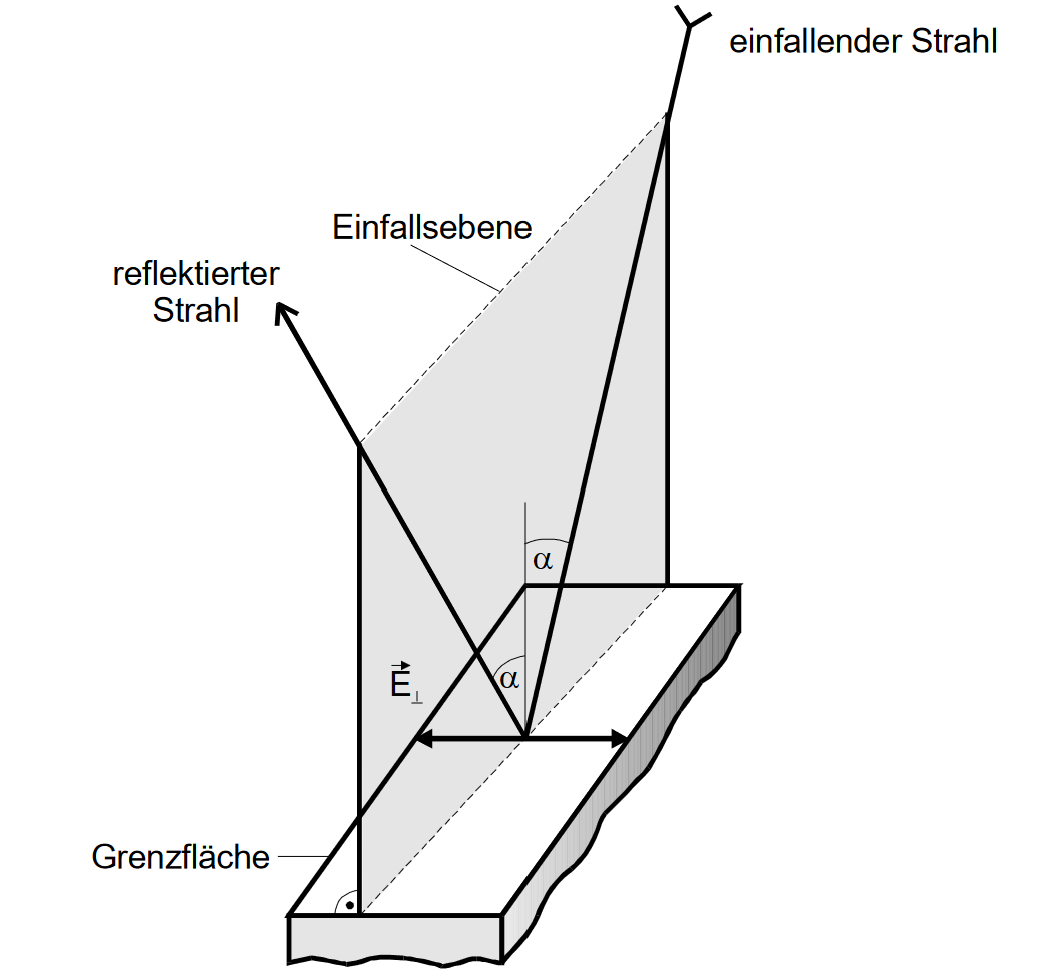
\includegraphics[width=0.6\linewidth]{content/grafik/bild1.png}
	\caption{Reflexion und Brechung des senkrecht polarisierten Lichtstrahls. \cite{fresnel}}
	\label{fig:bild1}
\end{figure}

Da die Beträge der $\vec{E}_{\perp}$ gleich ihren Tangentialkomponenten sind und keine Normalkomponente vorhanden ist kann aus den
Stetigkeitsbedingungen die Beziehung 
\begin{equation*}
    \vec{E}_{e\perp} + \vec{E}_{r \perp} = \vec{E}_{d\perp}
\end{equation*}
aufgestellt werden.  
Zusammen mit dem Snellius Brechungsgesetz
\begin{equation}
    n = \frac{\sin \alpha}{\sin \beta}
    \label{eqn:snellius}
\end{equation}
ergeben sich die Fresnel Formeln
\begin{equation}
    \begin{aligned}
    \vec{E}_{\mathrm{r}_{\perp}}&=-\vec{E}_{\mathrm{e}_{\perp}} \frac{\sin (\alpha-\beta)}{\sin (\alpha+\beta)} \quad \text{und}\\
    \vec{E}_{\mathrm{r}_{\perp}}&=-\vec{E}_{\mathrm{e}_{\perp}} \frac{\left(\sqrt{\mathrm{n}^2-\sin ^2 \alpha}-\cos \alpha\right)^2}{\mathrm{n}^2-1} .
    \label{eqn:fresnel1}
    \end{aligned}
\end{equation}

Für den streifenden Einfall $\alpha = \frac{\pi}{2}$ gilt
\begin{equation*}
    \vec{E}_{r\perp}(\frac{\pi}{2}) = - \vec{E}_{r\perp}.
\end{equation*}
Wenn der Lichtstrahl senkrecht einfällt, also bei $\alpha = 0$ gilt
\begin{equation*}
    \vec{E}_{r\perp}(0) = - \vec{E}_{r\perp}\frac{n - 1}{n + 1}.
\end{equation*}


Die Reflexion und Brechung des parallel zur Einfallsebene einfallenden Strahls ist in \autoref{fig:bild2} dargestellt.

\begin{figure}[H]
	\centering
	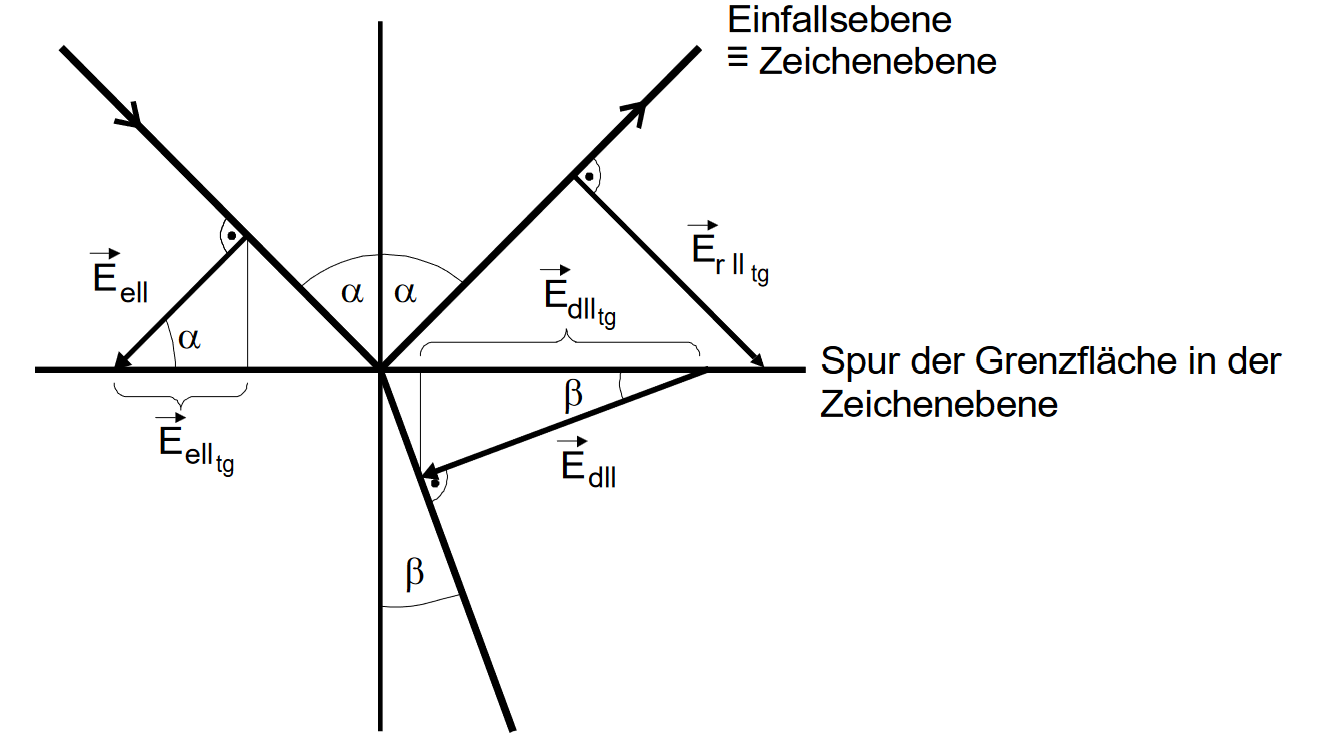
\includegraphics[width=0.9\linewidth]{content/grafik/bild2.png}
	\caption{Reflexion und Brechung des parallel polarisierten Lichtstrahls. \cite{fresnel}}
	\label{fig:bild2}
\end{figure}

Die parallel polarisierte Komponente $\vec{E}_{\|}$ setzt sich zusammen aus einer tangentialen Komponente $\vec{E}_{\|tg}$
und eine Komponente, welche normal zu Grenzfläche ist.

Aus den Stetigkeitsbedingungen und den Tangentialkomponenten der Vektoren $\vec{E}_{e\|}$, $\vec{E}_{r\|}$ und $\vec{E}_{d\|}$
ergibt sich die Gleichung
\begin{equation}
    \vec{E}_{r\|} = \vec{E}_{e\|} \frac{n \cos \alpha - \cos \beta}{n \cos \alpha + \cos \beta}.
    \label{eqn:keinname}
\end{equation}
Für das parallel polarisierte Licht lassen sich ebenfalls die Fresnelschen Gleichungen aufstellen
\begin{equation}
    \begin{aligned}
    \vec{E}_{r \|}&=\vec{E}_e \| \frac{\tan (\alpha-\beta)}{\tan (\alpha+\beta)} \quad \text{und}\\
    \vec{E}_{r \|}(\alpha)&=\vec{E}_e \| \frac{n^2 \cos \alpha-\sqrt{n^2-\sin ^2 \alpha}}{n^2 \cos \alpha+\sqrt{n^2-\sin ^2 \alpha}} .
    \label{eqn:fresnel2}
    \end{aligned}
\end{equation}
Für den senkrechten Einfall $ \alpha = 0$ gilt
\begin{equation*}
    \vec{E}_{r\|}(0) = \vec{E}_{e\|} \frac{n - 1}{n + 1}
\end{equation*}
und für den streifenden Fall $\alpha= \frac{\pi}{2}$ gilt
\begin{equation*}
    \vec{E}_{r\|}(\frac{\pi}{2}) = -\vec{E}_{e\|}.
\end{equation*}

Fällt Licht unter einem Winkel $\alpha_0$, dem sogenannten Brewsterschen Winkel, auf die Grenzfläche, so wird dieses
nicht mehr reflektiert sondern dringt ganz in das brechende Medium ein.
